%This chapter introduces the SM and the important interactions
%Then top physics is introduced talking about the decay
%tW and tt bar and their crosssections
%What is NLO and LO when are the diagrams similar
%Motivate the difficulties




\chapter{The Standard Model of Particle Physics}
\label{chp:sm}

Originally in an attempt do unify the electromagnetic, weak and strong force under one theory the standard model of particle physics represents the status quo of particle physics summarizing the elementary particles and their interactions.
The model is a gauge quantum field theory and its eternal symmetry is the unitary product group $SU(3) \times SU(2) \times U(1)$ in which the interactions are represented by particles named gauge bosons.

Although failing to answer open questions like the origin of dark matter or neutrino oscillations the Standard Model is a powerful model and has been successful in providing experimental predictions for decades.

\begin{figure}
	\centering
	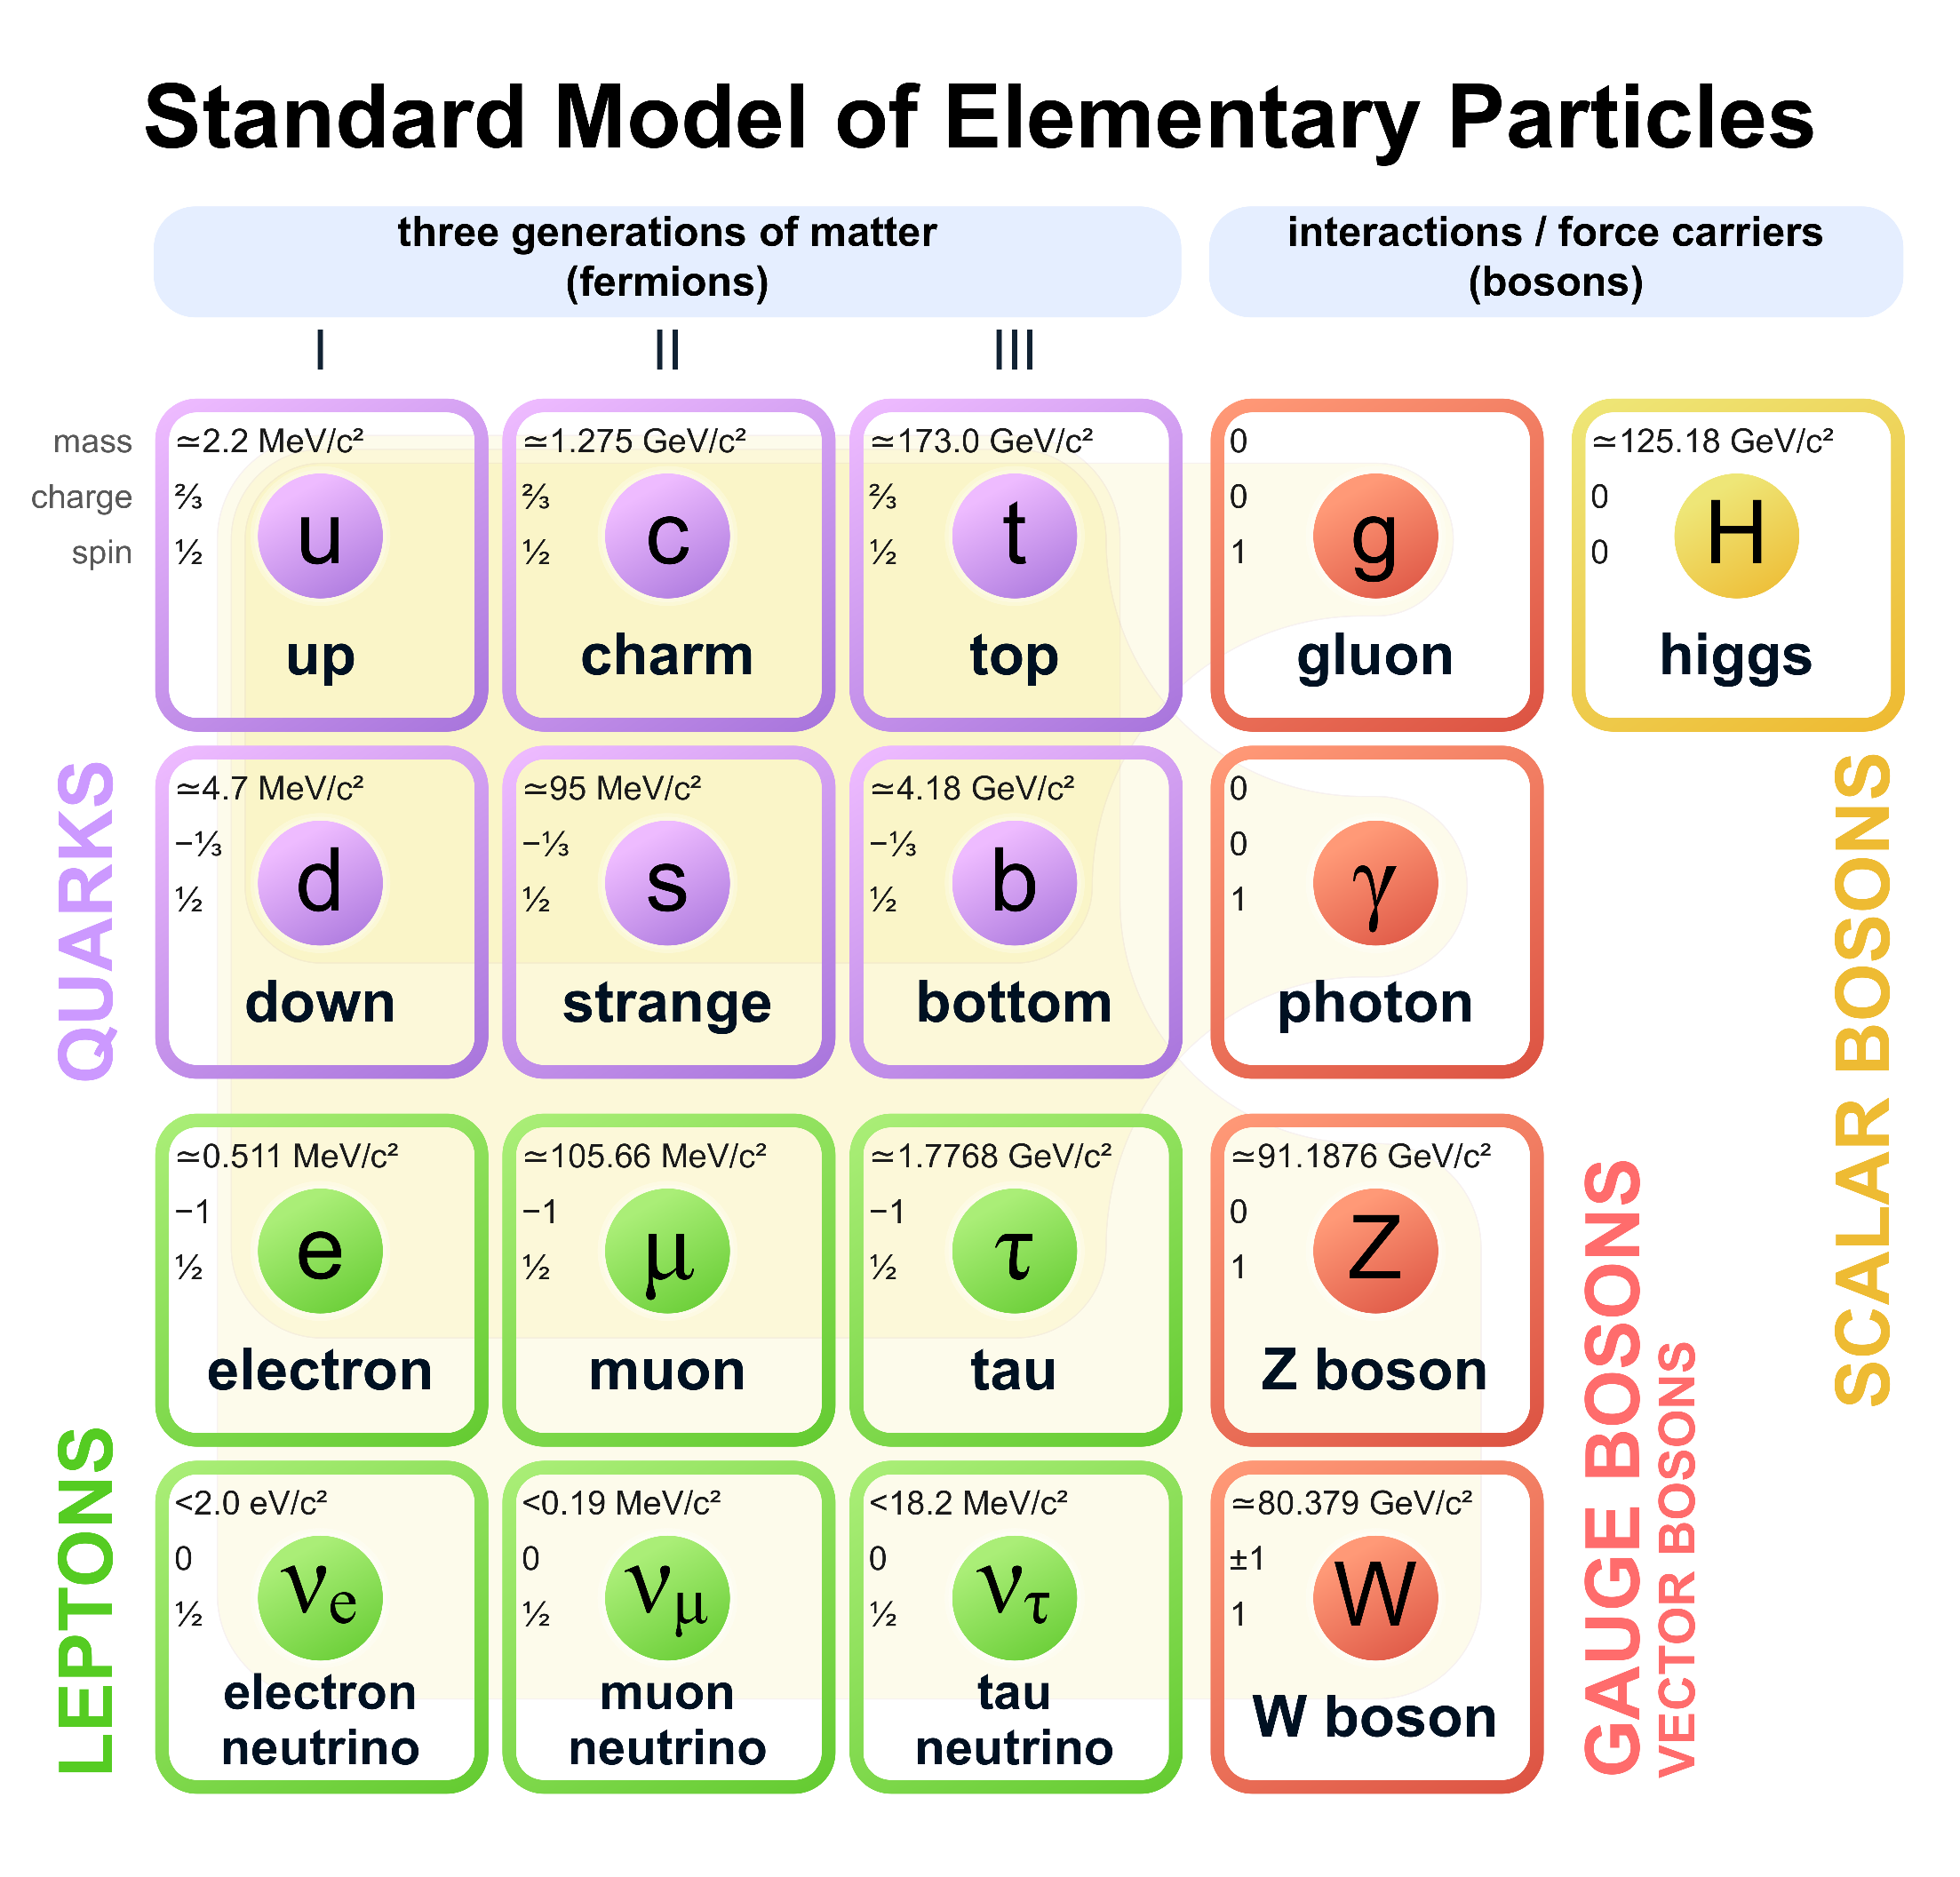
\includegraphics[width=\textwidth]{figures_SM/standard_model.eps}
	\caption[Standard Model particles]{Summary table of the Standard Model particles and their properties. The sketch~\cite{standard_model} was updated to PDG 2018 data~\cite{PDG}}
	\label{fig:sm}
\end{figure}



\section{Interactions}

\section{Particles}

\begin{align}
\begin{pmatrix}
\Pdown^{\prime} \\
\Pstrange^{\prime} \\
\Pbottom^{\prime}
\end{pmatrix}
=
\begin{pmatrix}
\Vud & \Vus & \Vub \\
\Vcd & \Vcs & \Vcb \\
\Vtd & \Vts & \Vtb \\
\end{pmatrix}
\cdot
\begin{pmatrix}
\Pdown \\
\Pstrange \\
\Pbottom
\end{pmatrix}
\end{align}

\section{Top physics}

For more information about the standard model see ~\cite{thomson, griffiths}